\documentclass[tikz,border=8pt]{standalone}
\usepackage{tikz}
\usetikzlibrary{shapes,arrows,positioning}
\tikzstyle{proc}=[rectangle,draw,rounded corners,fill=blue!10,align=center,minimum width=3.4cm,minimum height=0.9cm,font=\small]
\tikzstyle{dec}=[diamond,draw,fill=green!10,align=center,aspect=2,font=\small]
\tikzstyle{term}=[rectangle,draw,rounded corners=8pt,fill=gray!15,align=center,minimum width=2.6cm,minimum height=0.9cm,font=\small\bfseries]
\tikzstyle{arr}=[->,thick]
\begin{document}
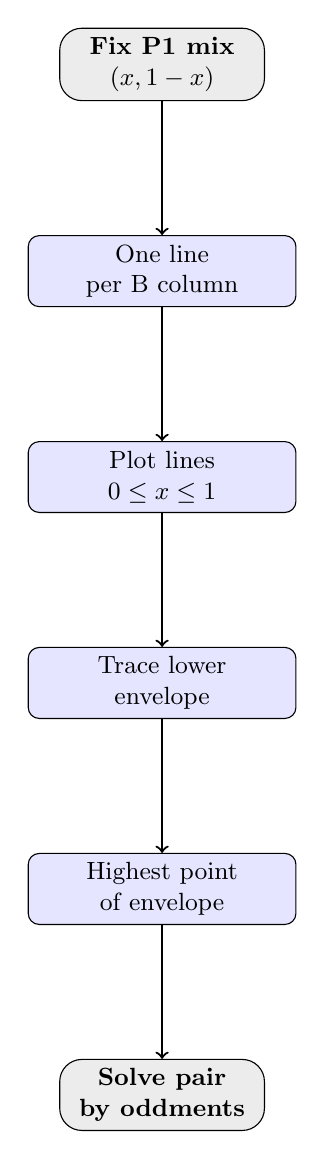
\begin{tikzpicture}[node distance=1.7cm]
\node[term] (A) {Fix P1 mix\\$(x,1-x)$};
\node[proc, below=of A] (B) {One line\\per B column};
\node[proc, below=of B] (C) {Plot lines\\$0 \le x \le 1$};
\node[proc, below=of C] (D) {Trace lower\\envelope};
\node[proc, below=of D] (E) {Highest point\\of envelope};
\node[term, below=of E] (F) {Solve pair\\by oddments};
\draw[arr] (A) -- (B);
\draw[arr] (B) -- (C);
\draw[arr] (C) -- (D);
\draw[arr] (D) -- (E);
\draw[arr] (E) -- (F);
\end{tikzpicture}
\end{document}
